\documentclass[border=10pt]{standalone}

\usepackage{tikz}
\usepackage{tikzsymbols}
\usetikzlibrary{calc,patterns,shapes.geometric}

\def\centerarc[#1](#2)(#3:#4:#5){\draw[#1] ($(#2)+({#5*cos(#3)},{#5*sin(#3)})$) arc (#3:#4:#5);}

\begin{document}
	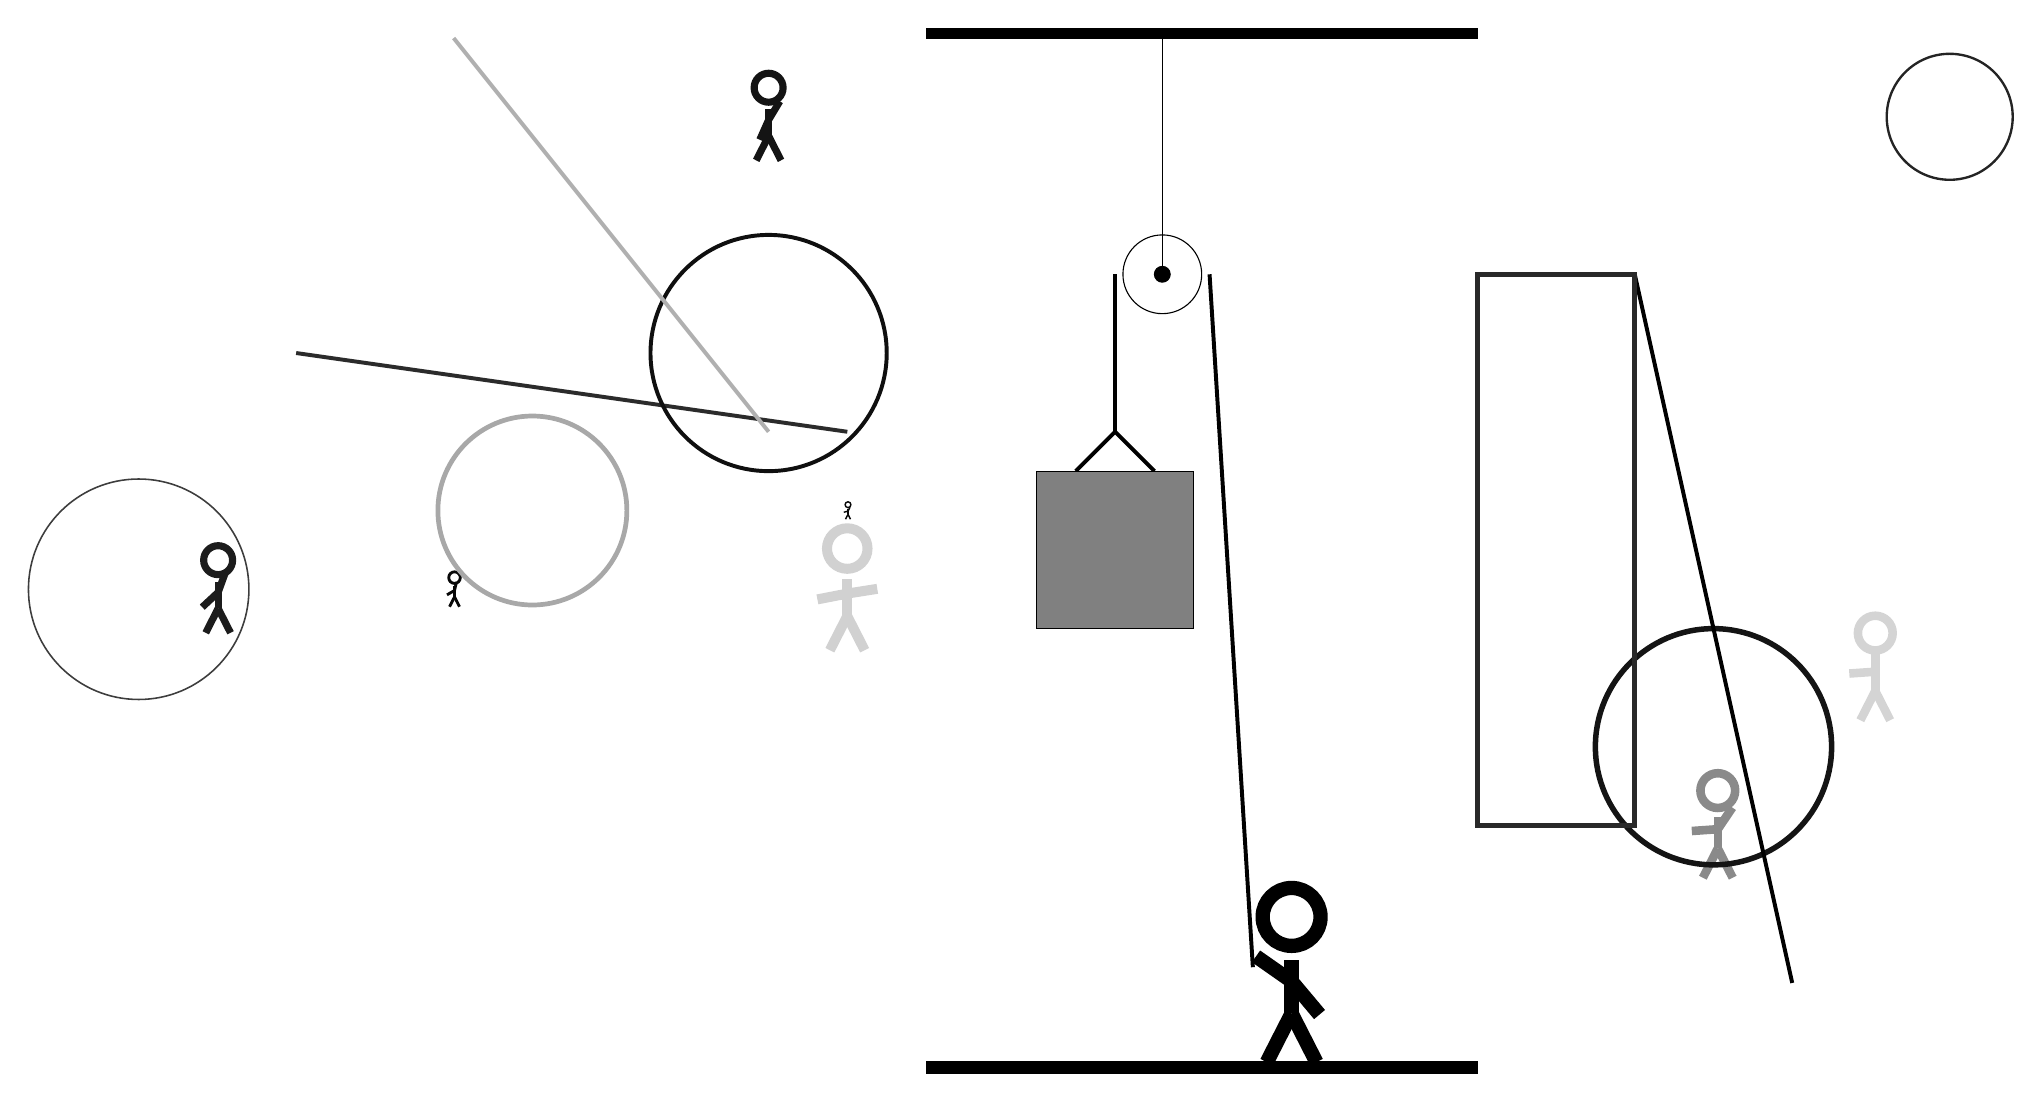
\begin{tikzpicture}
		%%%%% START %%%%%
		
		\draw[fill=black] (-2, 10) rectangle (5, 10.125);
		
		\draw[line width=0.5mm, color=black!83](-3, 5) -- (-10, 6);
		
		\draw [line width=0.3mm, color=black!86](11, 9) circle (0.8);
		\draw [line width=0.5mm, color=black!94](-4, 6) circle (1.5);
		\node[line width=0.6mm, color=black!97] at (-3, 4) {\Strichmaxerl[1][15][63]};
		\node[line width=0.5mm, color=black!18] at (-3, 3) {\Strichmaxerl[7][11][9]};
		
		\node[line width=0.3mm, color=black!46] at (8, 0) {\Strichmaxerl[6][4][56]};
		
		\node[line width=0.6mm, color=black!97] at (-8, 3) {\Strichmaxerl[2][30][77]};
		
		\draw [line width=0.7mm, color=black!92](8, 1) circle (1.5);
		\node[line width=0.2mm, color=black!92] at (-4, 9) {\Strichmaxerl[5][66][59]};
		
		\draw [line width=0.2mm, color=black!76](-12, 3) circle (1.4);
		\node[line width=0.5mm, color=black!17] at (10, 2) {\Strichmaxerl[6][4][90]};
		\draw[line width=0.5mm, color=black!100](9, -2) -- (7, 7);
		\draw [line width=0.6mm, color=black!34](-7, 4) circle (1.2);
		
		\node[line width=0.6mm, color=black!89] at (-11, 3) {\Strichmaxerl[5][43][70]};
		\draw[line width=0.5mm, color=black!31](-4, 5) -- (-8, 10);
		\draw[line width=0.6mm, color=black!84] (7, 7) rectangle (5, 0);
		
		
		\draw (1, 7) circle (0.5);
		\draw[fill=black] (1, 7) circle (0.1);
		\draw (1, 10) -- (1, 7);
		
		\draw[line width=0.5mm] (-0.1, 4.5) -- (0.4, 5.0) -- (0.9, 4.5);
		\draw[fill=black!50] (-0.6, 4.5) rectangle (1.4, 2.5);
		
		\draw[line width=0.5mm] (0.4, 7) -- (0.4, 5.0);
		\centerarc[line width=0.5mm](1, 7)(0:180:0.6);
		\draw[line width=0.5mm](1.6, 7) -- (2.15, -1.8);
		
		\node at (2.6, -1.9) {\Strichmaxerl[10][-35][-50]};
		
		\draw[fill=black] (-2, -3) rectangle (5, -3.15);
		
		%%%%% END %%%%%
	\end{tikzpicture}
\end{document}